\documentclass{article}

\textwidth=6.5in
\textheight=8.5in
\voffset=-54pt
\oddsidemargin=0in
\evensidemargin=0in
\setlength{\parskip}{8pt}
\setlength{\parindent}{0pt}

\usepackage{workbook}

\usepackage[]{handout}

\begin{document}

\begin{center}
\large\textsc{Problem Set 21 - The Definite Integral}
  
      \pspace{12pt}
  \begin{problemonly}\large Name: \rule{5cm}{0.15mm}\\ \end{problemonly}
\end{center}


\begin{grading}
\begin{enumerate}
    \item 12 points
    \item 10 points
    \item 10 points
    \item 15 points
    \item 5 points
\end{enumerate}
Total: 52 points.
\end{grading}

\begin{enumerate}
 

\item 

\begin{grading}
12 points. 3 for each part.
\end{grading}

 For help with the following, skim pp. 725-729 in Gottlieb, and read the examples on pp. 731-737.
 
Evaluate the following definite integrals by interpreting each as a
  signed area. Include a labeled graph to explain how you arrived at your answers.

  \probonly{}
    \begin{enumerate}
    \item
      \begin{problem}[\vfill]
        $\displaystyle \int_{-1}^{3}3\, dx$
      \end{problem}

      \begin{solution} % Jason Bland
        This is the signed area under $y = 3$ from $x = -1$ to $x = 3$.
        That region is a rectangle above the $x$-axis of height 3 and
        width $3 - (-1) = 4$, so the signed area is $\boxed{12}$.
      \end{solution}

    \item
      \begin{problem}[\vfill]
        $\displaystyle\int_{-2}^5 | x-2 | \, dx$
      \end{problem}

      \begin{solution} % Jason Bland
        We can picture this as the following signed area:
        \begin{center}
          \begin{tikzpicture}
            \begin{axis}[axis equal=true, xtick={-2, 2, 5}, width=3in]
              \addplot+[domain=-2:5, plusarea] {abs(x - 2)} \closedcycle;
              \addplot+[domain=-2.5:5.5, black] {abs(x - 2)} node[left]{$y
                = |x - 2|$};
            \end{axis}
          \end{tikzpicture}
        \end{center}        
        There are two triangles contributing to the area; one having base
        and height 4 (so area 8), the other having base and height 3 (so
        area $9/2$). The total area is $\boxed{\frac{25}{2}}$.
      \end{solution}

    \item
      \begin{problem}[\vfill] % Jason Bland
        $\displaystyle \int_{-2}^5 (|x| - 2) \, dx$
      \end{problem}

      \begin{solution}
        We can picture this as the following signed area:
        \begin{center}
          \begin{tikzpicture}
            \begin{axis}[axis equal=true, xtick={-2, 2, 5}, width=3in]
              \addplot+[domain=-2:2, minusarea] {abs(x) - 2} \closedcycle;
              \addplot+[domain=2:5, plusarea] {abs(x) - 2} \closedcycle;
              \addplot+[domain=-2.5:5.5, black] {abs(x) - 2} node[left]{$y
                = |x| - 2$};
            \end{axis}
          \end{tikzpicture}
        \end{center}                
        The green triangle has width and height 3, so its area is
        $\frac{9}{2}$.  The red triangle has width 4 and height 2, so its
        area is 4. Therefore, the total signed area is $\displaystyle
        \frac{9}{2} - 4 = \boxed{\frac{1}{2}}$.
      \end{solution}

    \item
      \begin{problem}[\vfill\newpage] % Jason Bland
        $\displaystyle \int_{-3}^3 \arctan(x) \, dx$
      \end{problem}

      \begin{solution}
        We can picture this as the following signed area:
        \begin{center}
          \begin{tikzpicture}
            \begin{axis}[width=3in, height=1.75in, xtick={-3, 3},
              ytick=\empty] 
              \addplot+[domain=-3:0, minusarea] {rad(atan(x))}
              \closedcycle; 
              \addplot+[domain=0:3, plusarea] {rad(atan(x))}
              \closedcycle;
              \addplot+[domain=-5:5, black] {rad(atan(x))};
            \end{axis}
          \end{tikzpicture}
        \end{center}
        The green and red regions are identically shaped, so their areas
        cancel each other, and the total signed area is $\boxed{0}$. 
      \end{solution}

    \end{enumerate}
  \probonly{}

\item

\begin{grading}
10 points. Students should receive little to no credit if they do not include graphs of the integrals, or if they attempt to evaluate the integral using antiderivatives.
\end{grading}

Put the following six integrals in ascending order, placing ``$<$'' or
  ``$=$'' signs between them as appropriate. Use labeled graphs to explain your answer. \textbf{Please note that you should be able to complete this problem without using any calculators or finding the exact values of the integrals!}

  
    \begin{enumeratecols}{3}
    \item $\displaystyle \int_{0}^{\pi}\sin(t)\, dt$
    \item $\displaystyle \int_{-\pi}^{2\pi}\sin(t)\, dt$
    \item $\displaystyle \int_{-\pi}^{2\pi}\cos(t) \,dt$
    \item $\displaystyle \int_{0}^{\pi/2}\cos(t) \,dt$
    \item $\displaystyle \int_{0}^{\pi}\cos(2t) \,dt$
    \item $\displaystyle \int_{0}^{3\pi/2}|\sin(t)|\,dt$
    \end{enumeratecols}

  \pspace{\newpage}

  \begin{solution} % Jason Bland
    We can visualize each integral as a signed area: 

    \begin{enumerate}
    \item 
      \raisebox{2ex-\height}{
        \begin{tikzpicture}
          \begin{axis}[axis equal image, xmax=6.283, xtick={-3.142, -1.571, ..., 6.3}, xticklabels={$-\pi$, $-\frac{\pi}{2}$, $0$, $\frac{\pi}{2}$, $\pi$, $\frac{3 \pi}{2}$, $2 \pi$}]
            \addplot+[domain=0:pi, plusarea] {sin(deg(x))} \closedcycle;
            \addplot+[domain=-pi:2 * pi, black] {sin(deg(x))};
        \end{axis}
        \end{tikzpicture}
      }

    \item       
      \raisebox{2ex-\height}{
        \begin{tikzpicture}
          \begin{axis}[axis equal image, xmax=6.283, xtick={-3.142, -1.571, ..., 6.3}, xticklabels={$-\pi$, $-\frac{\pi}{2}$, $0$, $\frac{\pi}{2}$, $\pi$, $\frac{3 \pi}{2}$, $2 \pi$}]
            \addplot+[domain=0:pi, plusarea] {sin(deg(x))} \closedcycle;
            \addplot+[domain=-pi:0, minusarea] {sin(deg(x))} \closedcycle;
            \addplot+[domain=pi:2 * pi, minusarea] {sin(deg(x))} \closedcycle;
            \addplot+[domain=-pi:2 * pi, black] {sin(deg(x))};
          \end{axis}
        \end{tikzpicture}
      }

    \item       
      \raisebox{2ex-\height}{
        \begin{tikzpicture}
          \begin{axis}[axis equal image, xmax=6.283, xtick={-3.142, -1.571, ..., 6.3}, xticklabels={$-\pi$, $-\frac{\pi}{2}$, $0$, $\frac{\pi}{2}$, $\pi$, $\frac{3 \pi}{2}$, $2 \pi$}]
            \addplot+[domain=-0.5 * pi:0.5 * pi, plusarea] {cos(deg(x))} \closedcycle;
            \addplot+[domain=-pi:-0.5 * pi, minusarea] {cos(deg(x))} \closedcycle;
            \addplot+[domain=0.5 * pi:1.5 * pi, minusarea] {cos(deg(x))} \closedcycle;
            \addplot+[domain=1.5 * pi : 2 * pi, plusarea] {cos(deg(x))} \closedcycle;
            \addplot+[domain=-pi:2 * pi, black] {cos(deg(x))};
          \end{axis}
        \end{tikzpicture}
      }

    \item       
      \raisebox{2ex-\height}{
        \begin{tikzpicture}
          \begin{axis}[axis equal image, xmax=6.283, xtick={-3.142, -1.571, ..., 6.3}, xticklabels={$-\pi$, $-\frac{\pi}{2}$, $0$, $\frac{\pi}{2}$, $\pi$, $\frac{3 \pi}{2}$, $2 \pi$}]
            \addplot+[domain=0:pi/2, plusarea] {cos(deg(x))} \closedcycle;
            \addplot+[domain=-pi:2 * pi, black] {cos(deg(x))};
          \end{axis}
        \end{tikzpicture}
      }

    \item       
      \raisebox{2ex-\height}{
        \begin{tikzpicture}
          \begin{axis}[axis equal image, xmax=6.283, xtick={-3.142, -1.571, ..., 6.3}, xticklabels={$-\pi$, $-\frac{\pi}{2}$, $0$, $\frac{\pi}{2}$, $\pi$, $\frac{3 \pi}{2}$, $2 \pi$}]
            \addplot+[domain=0:0.25 * pi, plusarea] {cos(2 *deg(x))} \closedcycle;
            \addplot+[domain=0.25 * pi:0.75 * pi, minusarea] {cos(2 * deg(x))} \closedcycle;
            \addplot+[domain=0.75 * pi : pi, plusarea] {cos(2 * deg(x))} \closedcycle;
            \addplot+[domain=-pi:2 * pi, black] {cos(2 * deg(x))};
          \end{axis}
        \end{tikzpicture}
      }

    \item       
      \raisebox{2ex-\height}{
        \begin{tikzpicture}
          \begin{axis}[axis equal image, xmax=6.283, xtick={-3.142, -1.571, ..., 6.3}, xticklabels={$-\pi$, $-\frac{\pi}{2}$, $0$, $\frac{\pi}{2}$, $\pi$, $\frac{3 \pi}{2}$, $2 \pi$}]
            \addplot+[domain=0:1.5 * pi, plusarea] {abs(sin(deg(x)))} \closedcycle;
            \addplot+[domain=-pi:2 * pi, black] {abs(sin(deg(x)))};
            \addplot+[domain=pi:2*pi, white] {-1};
          \end{axis}
        \end{tikzpicture}
      }
    \end{enumerate}

    We see that (b) is negative, while (c) and (e) are zero. The area in
    (a) is twice the area in (d), while the area in (f) is three times the
    area in (d). So, $\boxed{(\text{b}) < (\text{c}) = (\text{e}) <
      (\text{d}) < (\text{a}) < (\text{f})}$.
  \end{solution}

% \item ({Problem Set 20}, {{\#3}})

%  (22.3.7) % 22.3.7

%   \begin{enumerate}

%   \item
%     \begin{problem}
%       What is the equation of a circle of radius 2 centered at the origin?
%     \end{problem}

%     \begin{solution}
%       $x^2 + y^2 = 2^2$.
%     \end{solution}

%   \item
%     \begin{problem}
%       Write a function, complete with domain, that gives the equation of
%       the top half of a circle of radius 2 centered at the origin.
%     \end{problem}

%     \begin{solution}
%       The top half of the circle is the part with $y \geq 0$, so we just
%       solve the equation $x^2 + y^2 = 4$ for these $y$:
%       \begin{align*}
%         y^2 &= 4 - x^2 \\
%         \Aboxed{y &= \sqrt{4 - x^2} }
%       \end{align*}
%       (We use the positive square root because we want $y \geq 0$.)
%     \end{solution}

%   \item
%     \begin{problem}
%       Let $f(x) = \begin{cases}
%         \sqrt{4-x^2}& \text{ for } -2\le
%         x\le 0,\\
%         2x&\text{ for } x > 0.\\
%       \end{cases}$

%       Evaluate $\displaystyle \int_{-2}^{2} f(x)\, dx$.
%     \end{problem}

%     \begin{solution}
%       On $[-2, 0]$, the graph of $f$ is just part of the top half of the
%       circle of radius 2 centered at the origin.  Therefore, we can
%       picture $\displaystyle \int_{-2}^2 f(x)\,dx$ as the signed area below:
%       \begin{center}
%         \begin{tikzpicture}
%           \begin{axis}[width=2.5in, cycle list=black, axis equal=true, height=3in]
%             \addplot+[plusarea, domain=-2:0] {sqrt(4-x^2)} \closedcycle;
%             \addplot+[plusarea, domain=0:2] {2*x} \closedcycle;
%             \addplot+[domain=-2:0] {sqrt(4-x^2)};
%             \addplot+[domain=0:2.5] {2*x};
%             \addplot+[open] coordinates { (0, 0) };
%             \addplot+[closed] coordinates { (0, 2) };
%           \end{axis}
%         \end{tikzpicture}
%       \end{center}
%       This area is
%       \[ \underbrace{\frac{1}{4} \cdot \pi \cdot 2^2}_{\text{quarter
%           circle of radius 2}} + \underbrace{\frac{1}{2} \cdot 2 \cdot
%         4}_{\text{triangle}} = \boxed{\pi + 4}.\]
%     \end{solution}

%   \end{enumerate}

\item 

\begin{grading}
10 points. 8 for part (a), 2 for part (b).
\end{grading}

\begin{enumerate}[topsep=0pt]
  \item
    \begin{problem}[\vfill]
      Find upper and lower bounds\footnote{Recall that ``upper bound'' is
        another way of saying ``overestimate'' and ``lower bound'' is
        another way of saying ``underestimate''.} for $\displaystyle
      \int_3^5 x^3\,dx$ using left-hand and right-hand sums with 4
      rectangles.  Please write your sums out longhand (e.g., $1^2 \cdot
      \frac{1}{3} + 5^2 \cdot \frac{1}{3} + 6^2 \cdot \frac{1}{3}$), and
      evaluate them.

      Use the Riemann sums applet at
      \url{https://www.geogebra.org/m/sgxnjavg} to check your
      answers.
    \end{problem}

    \begin{solution} % Jason Bland
      Here are pictures of $L_4$ and $R_4$.  (Since we're using 4
      rectangles on an interval of width 2, each rectangle will hvae width
      $0.5$.) 
      \begin{center}
        \begin{tabular}{ccc}
          \begin{tikzpicture}[declare function={f(\x) = \x^3;}]
            \begin{axis}[ymin=0, cycle list=black, ytick=\empty, xtick={3,
                3.5, 4, 4.5, 5}, hide y axis, width=3in]
              \addplot+[ybar interval, plusarea] coordinates {
                (3, {f(3)}) (3.5, {f(3.5)}) (4, {f(4)}) (4.5, {f(4.5)}) (5,
                {f(4.5)})
              };
              \addplot+[domain=2.75:5.25] { f(x) } node[left]{$y = x^3$};
            \end{axis}
          \end{tikzpicture}
          & \hspace{0.25in} &
          \begin{tikzpicture}[declare function={f(\x) = \x^3;}]
            \begin{axis}[ymin=0, cycle list=black, ytick=\empty, xtick={3,
                3.5, 4, 4.5, 5}, hide y axis, width=3in]
              \addplot+[ybar interval, plusarea] coordinates {
                (3, {f(3.5)}) (3.5, {f(4)}) (4, {f(4.5)}) (4.5,
                {f(5)}) (5, {f(5)})
              };
              \addplot+[domain=2.75:5.25] { f(x) } node[left]{$y = x^3$};
            \end{axis}
          \end{tikzpicture}          
          \\
          $L_4$ && $R_4$
        \end{tabular}
      \end{center}
      So, a lower bound is $L_4 = 3^3 \cdot 0.5 + 3.5^3 \cdot 0.5 + 4^3
      \cdot 0.5 + 4.5^3 \cdot 0.5 = 112.5$, and an upper bound is $R_4 =
      3.5^3 \cdot 0.5 + 4^3 \cdot 0.5 + 4.5^3 \cdot 0.5 + 5^3 \cdot 0.5 =
      161.5$.
    \end{solution}

  \item

    \note{This is just to get students to think about the notation a
      little bit before we go into more detail next class.  Notation tends
      to be one of the hardest things in the integration unit.}

    \begin{problem}[\newpage]
      (Exploratory) As you can see in the applet, when we do left-hand and
      right-hand approximations, we can label the $x$-values where the
      rectangles' edges lie as $x_0, x_1, x_2$, and so on.  We also often
      call the width of each rectangle $\Delta x$ (read as ``delta x'').

      If we write $f(x) = x^3$, which of the following is equal to $L_4$,
      the left-hand sum with 4 rectangles?  Which of the following is
      equal to $R_4$, the right-hand sum with 4 rectangles?
      \begin{enumerate}
      \item $f(x_0) \Delta x + f(x_1) \Delta x + f(x_2) \Delta x + f(x_3)
        \Delta x + f(x_4) \Delta x$
      \item $f(x_0) \Delta x + f(x_1) \Delta x + f(x_2) \Delta x + f(x_3)
        \Delta x$
      \item $f(x_1) \Delta x + f(x_2) \Delta x + f(x_3) \Delta x + f(x_4)
        \Delta x$
      \end{enumerate}      
    \end{problem}

    \begin{solution}
      ii is the left-hand sum; iii is the right-hand sum.  (In this
      example, $\Delta x = 0.5$, $x_0 = 3$, $x_1 = 3.5$, $x_2 = 4$, $x_3 =
      4.5$, and $x_4 = 5$.)
    \end{solution}

  \end{enumerate}

\item 

\begin{grading}
15 points, as follows: 2/2/3/2/3/1/2
\end{grading}

  The rate $r(t)$ at which liquid nitrogen is pumped in and out of a tank is
  shown in the graph below.  There are 30 cubic feet of liquid nitrogen in
  the tank at $t = 0$. Give exact answers to the following questions,
  using definite integrals where necessary. If your answer contains a
  definite integral, give an approximation.

  \begin{center}
    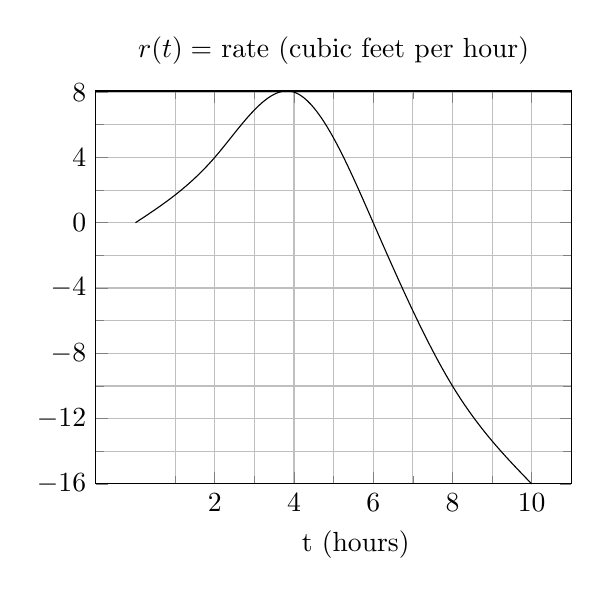
\begin{tikzpicture}
      \begin{axis}[xtick={2, 4, 6, 8, 10}, minor xtick={1, 3, 5, 7, 9},
        ytick={-16, -12, ..., 8}, minor ytick={-14, -10, ..., 6}, grid=both,
        enlarge y limits=false, clip=false, axis line style={shorten
          >=-8pt, shorten <=-8pt}, 
          title={$r(t)=$ rate (cubic feet per hour)},
          xlabel style={xshift=8pt}, xlabel=t (hours),width=3in]
        	\addplot[][domain=0:2]{+0.10047846889952153*x^3+-9.582200956937799e-61*x^2+1.5980861244019138*x^1+0*x^0};
			\addplot[][domain=2:4]{+-0.5023923444976076*x^3+3.617224880382775*x^2+-5.636363636363637*x^1+4.822966507177034*x^0};
			\addplot[][domain=4:6]{+0.4090909090909091*x^3+-7.320574162679426*x^2+38.11483253588517*x^1+-53.51196172248804*x^0};
			\addplot[][domain=6:8]{+0.11602870813397129*x^3+-2.0454545454545454*x^2+6.464114832535885*x^1+9.789473684210526*x^0};
			\addplot[][domain=8:10]{+-0.12320574162679426*x^3+3.6961722488038276*x^2+-39.4688995215311*x^1+132.2775119617225*x^0};
      \end{axis}
    \end{tikzpicture}      
  \end{center}


  \begin{enumerate}
  \item
    \begin{problem}[\vfill]
      How much liquid nitrogen flows into the tank between $t=2$ and $t=3$?
    \end{problem}

    \begin{solution}
      This is the net change between $t=2$ and $t=3$, or 
      $\boxed{\int_2^3 r(t)\,dt}$.
      
      Using rectangles to approximate the area under the graph, 
      a reasonable approximation would be \fbox{between
      $4$ and $7$ cubic feet.}
    \end{solution}

  \item
    \begin{problem}[\vfill]
      Is liquid nitrogen flowing into or out of the tank at $t = 8$?  At
      what rate? 
    \end{problem}

    \begin{solution}
      At $t=8$, liquid nitrogen is flowing 
      \fbox{out of the tank at $10$ cubic
      feet per hour}, since $r(8)=-10$.
    \end{solution}

  \item
    \begin{problem}[\vfill]
      How much liquid nitrogen is in the tank at $t=2$?
    \end{problem}

    \begin{solution}
      The net change between $t=0$ and $t=2$ is $\int_0^2 r(t)\,dt$. Since
      there are 30 cubic feet of liquid nitrogen in the tank at $t=0$, 
      the amount in the tank at $t=2$ would be 
      $\boxed{30+\int_0^2 r(t)\,dt.}$ 
      A reasonable approximation would be \fbox{between
      $32$ and $36$ cubic feet.}
    \end{solution}

  \item
    \begin{problem}[\vfill]
      At what time is liquid nitrogen flowing into the tank most quickly?
      How quickly is it flowing then?
    \end{problem}

    \begin{solution}
      The maximum of $r(t)$ occurs \fbox{at $t = 4$ or just prior}, and
      the maximum value is \fbox{$8$ cubic feet per hour.}
    \end{solution}

  \item
    \begin{problem}[\vfill\newpage]
      At what time is the amount of liquid nitrogen in the tank greatest?
      How much liquid nitrogen is in the tank then?
      (Your answers to parts (d) and (e) should be different.)
    \end{problem}

    \begin{solution}
      The amount of liquid nitrogen in the tank increases until $t=6$,
      after which it decreases. The maximum amount would occur at $t = 6$,
      equal to $\boxed{30+\int_0^6 r(t)\,dt}$. 
      A reasonable approximation would
      be \fbox{between $48$ and $64$ cubic feet.}
    \end{solution}

  \item
    \begin{problem}[\vfill]
      At what times is the amount of liquid nitrogen in the tank
      increasing?
    \end{problem}

    \begin{solution}
      On the interval $\boxed{0 \leq t \leq 6}$, since $r(t)$ is positive
      between $t=0$ and $t=6$.
    \end{solution}

  \item
    \begin{problem}[\vfill]
      At how many times between $t = 0$ and $t = 10$ is the amount of
      liquid nitrogen in the tank equal to 30 cubic feet?
    \end{problem}

    \begin{solution}
      The amount of liquid nitrogen in the tank increases from $t=0$ to
      $t=6$, then decreases until $t=10$. Since the portion of the area 
      under the curve below the horizontal axis is larger than the area 
      above the horizontal axis, there must be some time before $t=10$ when
      the amount of liquid nitrogen has decreased back to $30$ cubic feet.
      So \fbox{twice,} if we count $t=0$.
    \end{solution}

    % \begin{problem}[\newpage]
    %   Make a rough sketch of the volume $V(t)$ of liquid nitrogen in the
    %   tank as a function of time.  How are your answers to the previous
    %   parts reflected in your graph?
    % \end{problem}

    % \begin{solution}
    %   \begin{center}
    %     \begin{tikzpicture}
    %       \begin{axis}[cycle list=black, ytick={9, 33}]
    %         \addplot+[domain=0:4] {x^2 + 9}; %
    %         \addplot+[domain=4:10] {-2*x^2+24*x-39}; %
    %         \addplot+[closed] coordinates { (6, 33) } node[above] {$(6,
    %           33)$}; 
    %       \end{axis}
    %     \end{tikzpicture}
    %   \end{center}
    %   Key features:
    %   \begin{itemize}
    %   \item The graph starts out at the point $(0, 9)$ where its tangent
    %     line is horizontal.
    %   \item It's increasing and concave up for $0 < t < 4$, increasing and
    %     concave down for $4 < t < 6$, decreasing and concave down for $t >
    %     6$.
    %   \item Its absolute maximum point is $(6, 33)$. 
    %   \item The line $y = 10$ intersects the graph in two points (one of
    %     those is where $t = 1$). 
    %   \end{itemize}
    % \end{solution}

  \end{enumerate}

\item 

\begin{grading}
5 points. 
\end{grading}

\begin{problem}[\stretch{3}]
    {\bf Reflect Back.}  What characteristic of $f$ will ensure that a
    right hand sum gives an underestimate of $\displaystyle \int_a^b f(x)
    \, dx $?  Does it matter whether $f$ is positive or negative?
    Increasing or decreasing? Concave up or concave down?

    Illustrate your answer with some pictures.       
  \end{problem}

  \begin{solution}
    The function $f$ needs to be decreasing for this to be true, but the
    concavity does not matter:
    \begin{center}
      \begin{tikzpicture}[declare function={f(\x)=5*2^(-\x/4) + 1;}]
        \begin{axis}[hide y axis, ymin=0, xtick=\empty, width=2.5in]
          \addplot+[domain=0:8] {f(x)};
          \addplot+[ybar interval, plusarea] coordinates {
            (1, {f(2)}) (2, {f(3)}) (3, {f(4)}) (4, {f(5)}) (5, {f(6)})
            (6, {f(7)}) (7, {f(7)})
          };
        \end{axis}
      \end{tikzpicture}
      \hspace{0.25in}
      \begin{tikzpicture}[declare function={f(\x)=25-5*2^(\x/4);}]
        \begin{axis}[hide y axis, ymin=0, xtick=\empty, width=2.5in]
          \addplot+[domain=0:8] {f(x)};
          \addplot+[ybar interval, plusarea] coordinates {
            (1, {f(2)}) (2, {f(3)}) (3, {f(4)}) (4, {f(5)}) (5, {f(6)})
            (6, {f(7)}) (7, {f(7)})
          };
        \end{axis}
      \end{tikzpicture}
    \end{center}
    It's also true if the function is negative because the right-hand sum
    is then more negative than the actual integral:
    \begin{center}
      \begin{tikzpicture}[declare function={f(\x)=5*2^(-\x/4) - 6;}]
        \begin{axis}[hide y axis, ymax=0, xtick=\empty, width=2.5in]
          \addplot+[domain=0:8] {f(x)};
          \addplot+[ybar interval, minusarea] coordinates {
            (1, {f(2)}) (2, {f(3)}) (3, {f(4)}) (4, {f(5)}) (5, {f(6)})
            (6, {f(7)}) (7, {f(7)})
          };
        \end{axis}
      \end{tikzpicture}
      \hspace{0.25in}
      \begin{tikzpicture}[declare function={f(\x)=-5*2^(\x/4);}]
        \begin{axis}[hide y axis, ymax=0, xtick=\empty, width=2.5in]
          \addplot+[domain=0:8] {f(x)};
          \addplot+[ybar interval, minusarea] coordinates {
            (1, {f(2)}) (2, {f(3)}) (3, {f(4)}) (4, {f(5)}) (5, {f(6)})
            (6, {f(7)}) (7, {f(7)})
          };
        \end{axis}
      \end{tikzpicture}
    \end{center}
  \end{solution}

\end{enumerate}

\psreflection{
Optional reading for next class is \S 22.2 in Gottlieb.
}
\end{document}